\hypertarget{a00041}{\subsection{Client.\-View.\-Game\-Panel Klassenreferenz}
\label{a00041}\index{Client.\-View.\-Game\-Panel@{Client.\-View.\-Game\-Panel}}
}
Klassendiagramm für Client.\-View.\-Game\-Panel\-:\begin{figure}[H]
\begin{center}
\leavevmode
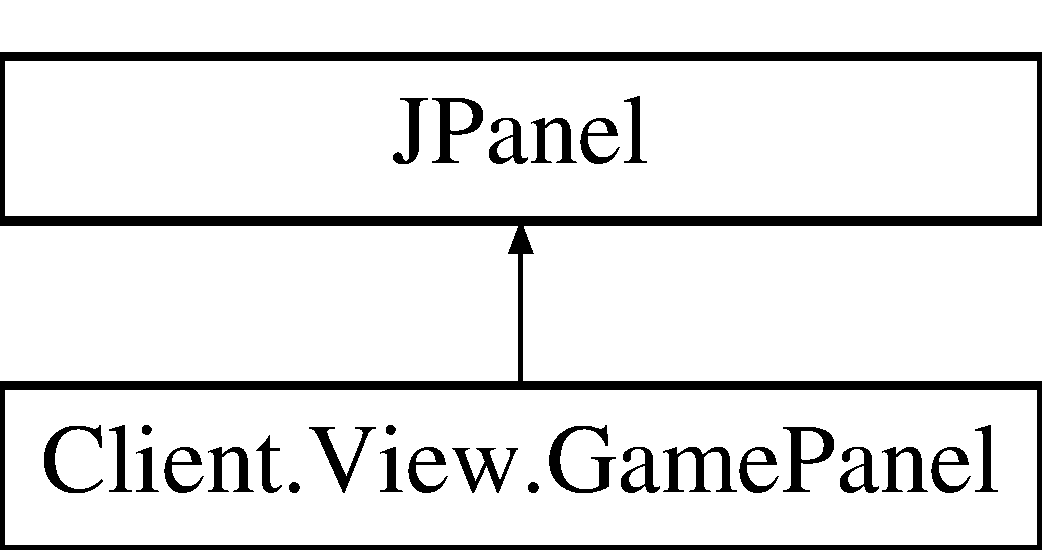
\includegraphics[height=2.000000cm]{a00041}
\end{center}
\end{figure}


\subsubsection{Ausführliche Beschreibung}
Es besteht aus veschiedenen Panelobjekten, welche je nach Regelwerk auf das Spielfeld gezeichnet werden. Dazu geh�ren die eigenen Karten, eventuell ausgew�hlte Karten, ein Textfeld z.\-B. zur Anzeige der Anzahl der restlichen Karten der Mitspieler und den Ablagestapel (/\-L194/). Nach jeder Runde wird der Punktestand aktualisiert.

\begin{DoxyAuthor}{Autor}
m4nkey 
\end{DoxyAuthor}
